\documentclass[t,11pt,aspectratio=169]{beamer}
\usepackage{tikz}
\usepackage{pgfplots}
\usetikzlibrary{calc}
\usepackage[utf8]{inputenc}
\usepackage[ngerman]{babel}
\usepackage{amsmath,amsfonts,amssymb}
\usepackage{framed}
\usecolortheme{orchid}
\usepackage{etoolbox}
\useinnertheme[shadow=true]{rounded}

\usepackage{verbatim}

%%% PROGRESSBAR
\definecolor{pbblue}{HTML}{D8D8D8}% filling color for the progress bar
\definecolor{pbgray}{HTML}{F2F2F2}% background color for the progress bar
\useoutertheme{infolines}
\setbeamerfont{footline}{size=\normalsize}
\setbeamersize{text margin left=30pt,text margin right=30pt}
\makeatletter
\setbeamertemplate{footline}
{
	\leavevmode%
	\hbox{%
		\begin{beamercolorbox}[wd=.333333\paperwidth,ht=2.5ex,dp=1ex,center]{title in head/foot}%
			\usebeamerfont{title in head/foot}\insertshorttitle
		\end{beamercolorbox}%
		\begin{beamercolorbox}[wd=.333333\paperwidth,ht=2.5ex,dp=1ex,center]{date in head/foot}%
			%\usebeamerfont{date in head/foot}\insertshortdate{}\hspace*{2em}
			%\insertframenumber\hspace*{2ex} 
		\end{beamercolorbox}
		\begin{beamercolorbox}[wd=.333333\paperwidth,ht=3ex,dp=1ex,center]{author in head/foot}%
			\usebeamerfont{author in head/foot}\insertshortauthor~~%\beamer@ifempty{\insertshortinstitute}{}{(\insertshortinstitute)}
		\end{beamercolorbox}%
	}%
	\vskip0pt%
}
\makeatother
\makeatletter
\def\progressbar@progressbar{} % the progress bar
\newcount\progressbar@tmpcounta% auxiliary counter
\newcount\progressbar@tmpcountb% auxiliary counter
\newdimen\progressbar@pbht %progressbar height
\newdimen\progressbar@pbwd %progressbar width
\newdimen\progressbar@tmpdim % auxiliary dimension
\progressbar@pbwd=\linewidth
\progressbar@pbht=1.5ex
\def\progressbar@progressbar{%
    \progressbar@tmpcounta=\insertpagenumber
    \progressbar@tmpcountb=\insertdocumentendpage
    \progressbar@tmpdim=\progressbar@pbwd
    \multiply\progressbar@tmpdim by \progressbar@tmpcounta
    \divide\progressbar@tmpdim by \progressbar@tmpcountb
  \begin{tikzpicture}[rounded corners=3pt,very thin]
    \shade[top color=pbgray!20,bottom color=pbgray!20,middle color=pbgray!50]
      (0pt, 0pt) rectangle ++ (\progressbar@pbwd, \progressbar@pbht);
      \shade[draw=pbblue,top color=pbblue!50,bottom color=pbblue!50,middle color=pbblue] %
        (0pt, 0pt) rectangle ++ (\progressbar@tmpdim, \progressbar@pbht);
    \draw[color=normal text.fg!50]  
      (0pt, 0pt) rectangle (\progressbar@pbwd, \progressbar@pbht) 
        node[pos=0.5,color=normal text.fg] {\textnormal{%
             \pgfmathparse{\insertpagenumber*100/\insertdocumentendpage}%
             \pgfmathprintnumber[fixed,precision=0]{\pgfmathresult}\,\%%
        }%
    };
  \end{tikzpicture}%
}
\addtobeamertemplate{headline}{}
{%
  \begin{beamercolorbox}[wd=\paperwidth,ht=4ex,center,dp=1ex]{white}%
    \progressbar@progressbar%
  \end{beamercolorbox}%
}
\makeatother

\setbeamertemplate{frametitle}[default][center]

%%% BLOCKS
% block = Aufgabe
\setbeamercolor{block title}{fg=black,bg=blue!30!white} 
\setbeamercolor{block body}{fg=black, bg=blue!3!white}

% alertblock = Definition
\setbeamercolor{block title alerted}{fg=black,bg=red!50!white} 
\setbeamercolor{block body alerted}{fg=black, bg=red!3!white}

% exampleblock = Wiederholung
\setbeamercolor{block title example}{fg=black,bg=green!30!white} 
\setbeamercolor{block body example}{fg=black, bg=green!3!white}

\setbeamercovered{transparent}
\setbeamertemplate{navigation symbols}{}

\addtocounter{page}{-1}
\addtocounter{framenumber}{-1}
\setbeamercovered{invisible}





\begin{document}
	
\begin{frame}
	\begin{itemize}
		\item \textbf{Odds-Ratio} und \textbf{Risk-Ratio} berechnen die Stärke eines möglichen Zusammenhanges zwischen einem Risikofaktor und einer Erkrankung.
		\item Besteht überhaupt ein Zusammenhang? Wie stark ist dieser Zusammenhang?
		\item Beide Maßzahlen sind häufig zu finden in medizinischen Studien.
	\end{itemize}
\end{frame}	
	
\begin{frame}
\begin{block}{Ein Beispiel:}
Uns liegt die folgende Kreuztabelle vor:
\begin{center}
	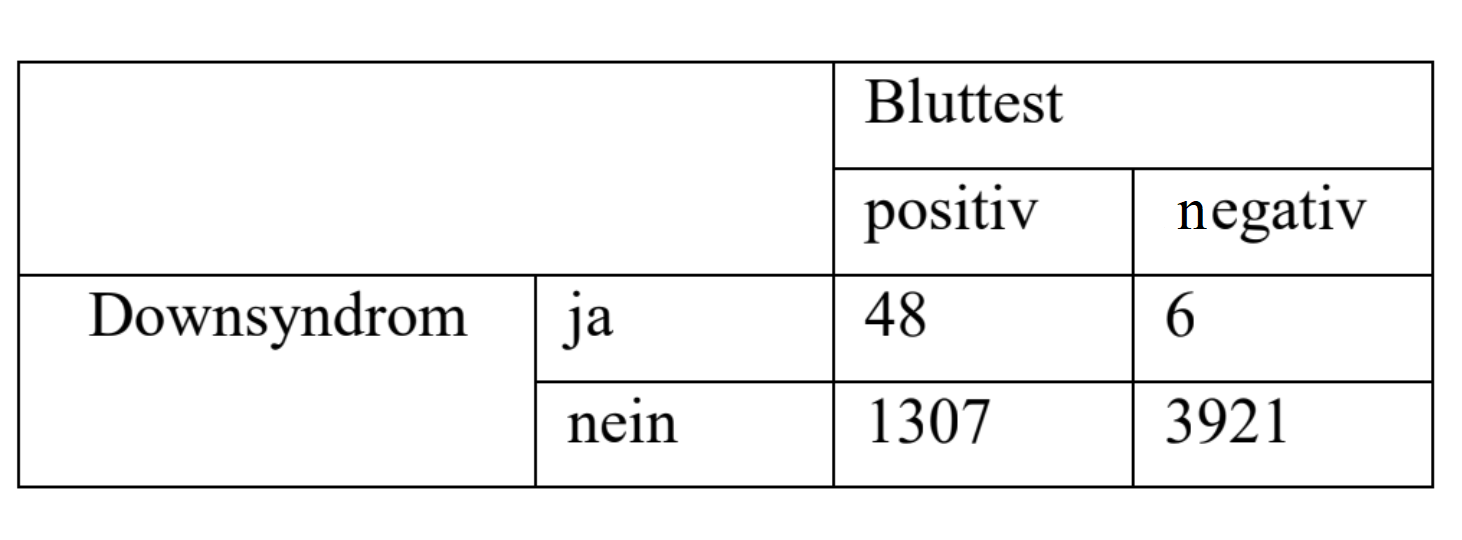
\includegraphics[scale=0.4]{tabelle.png}
\end{center}
Berechnen und interpretieren Sie die \textbf{Odds-Ratio} (das \textbf{Chancenverhältnis}).
\end{block}
\pause
\vfill
\textbf{Odds-Ratio:} Wie stark hängt ein vermuteter \textbf{Risikofaktor} mit einer \textbf{Erkrankung} zusammen?
\vfill
\end{frame}

\begin{frame}
\begin{center}
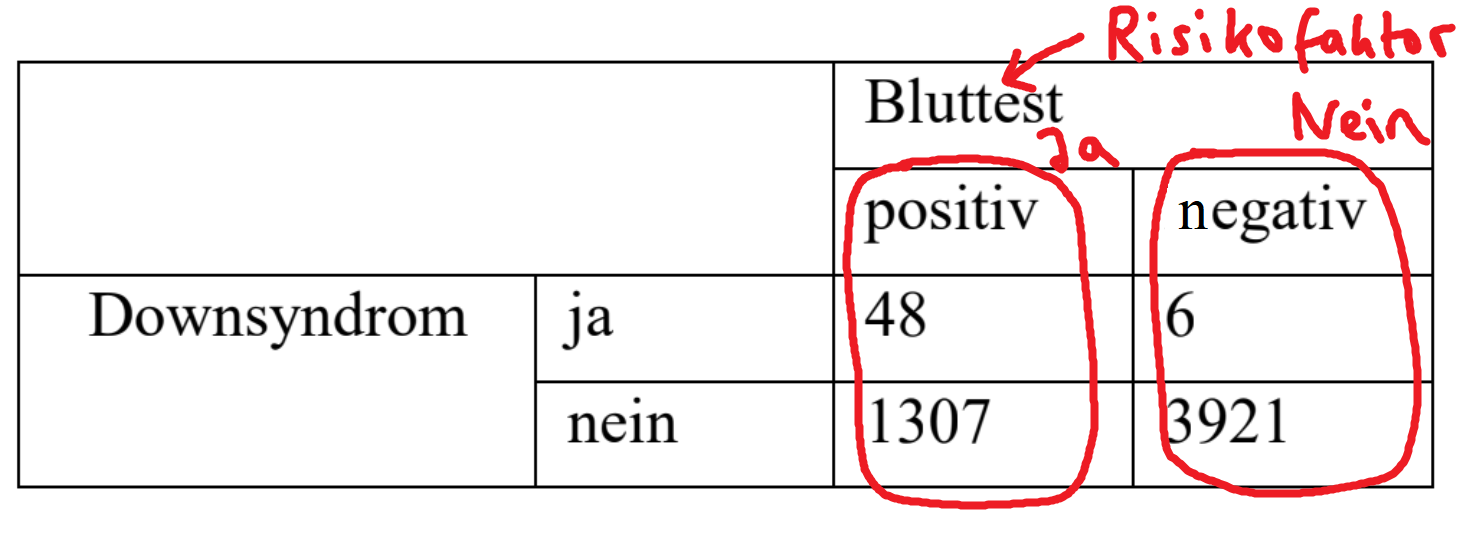
\includegraphics[width=\textwidth]{tabelle2.png}
\end{center}
\end{frame}

\begin{frame}
\begin{center}
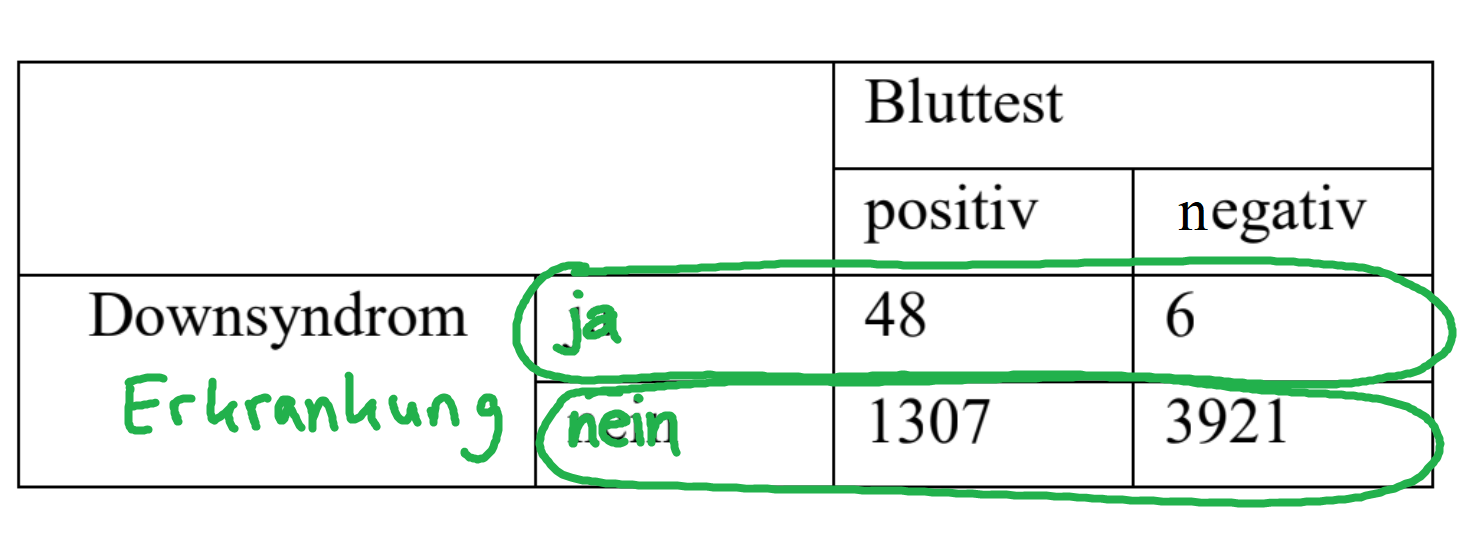
\includegraphics[width=\textwidth]{tabelle3.png}
\end{center}
\end{frame}

\begin{frame}
Der Unterschied zwischen \textbf{Odds} und \textbf{Wahrscheinlichkeit} (\textbf{Risiko}):
\begin{itemize}
	\item Odds = Wahrscheinlichkeit / Gegenwahrscheinlichkeit
	\item Die Wahrscheinlichkeit, dass bei einem Münzwurf Kopf erscheint, beträgt 0,5. Die Chance (Odds) beträgt 1 (1:1). 
	\item Bei der Berechnung der Wahrscheinlichkeit gehen alle Fälle in den Nenner ein (1/2), bei der Berechnung der Odds gehen nur die Fälle in den Nenner ein, die noch nicht im Zähler berücksichtigt wurden (1/1).
	\item Wahrscheinlichkeiten liegen zwischen 0 und 1, Odds hingegen liegen zwischen 0 und $\infty$.
\end{itemize}
\end{frame}

\begin{frame}
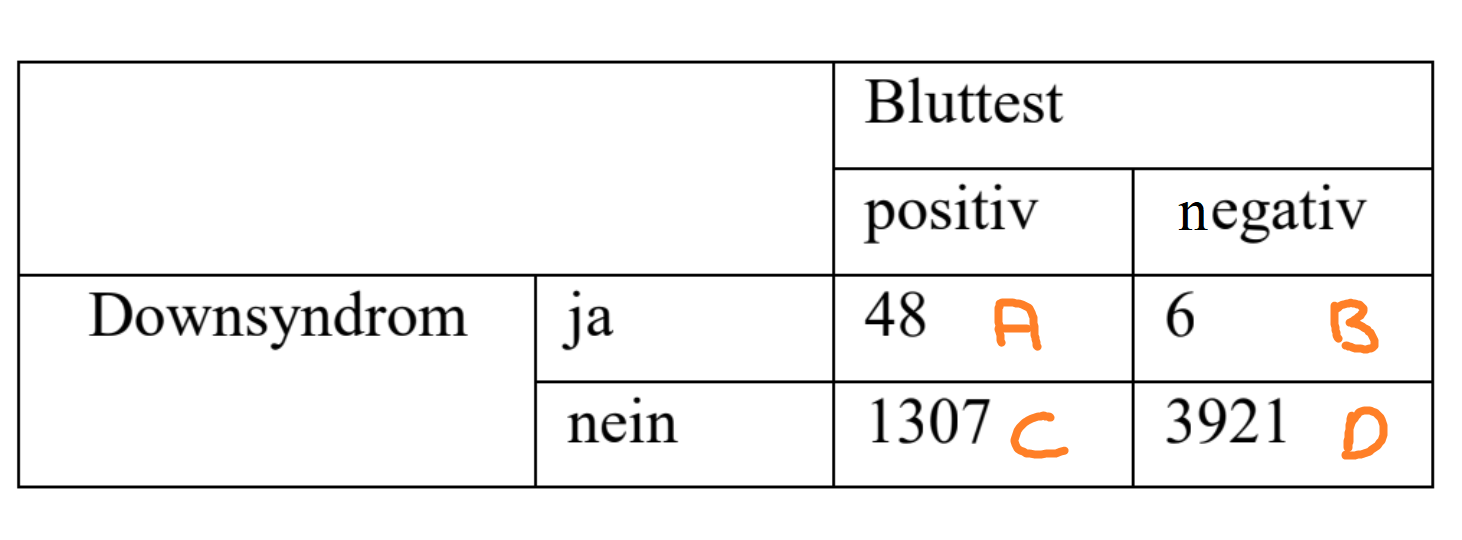
\includegraphics[width=\textwidth]{tabelle4.png}
\vfill
\textbf{Berechnung:}
\begin{align*}
\text{Odds-Ratio} = \frac{\text{Odds für Erkrankung mit Risikofaktor}}{\text{Odds für Erkrankung ohne Risikofaktor}} = \frac{\frac{A}{B}}{\frac{C}{D}} = \frac{A\cdot D}{B \cdot C} = \frac{48\cdot 3921}{6 \cdot 1307} = 24
\end{align*}
\vfill
\end{frame}

\begin{frame}
\textbf{Berechnung:}
\begin{align*}
\text{Odds-Ratio} = \frac{A\cdot D}{B \cdot C} = \frac{48\cdot 3921}{6 \cdot 1307} = 24
\end{align*}
\textbf{Interpretation:}
\begin{itemize}
\item Die Odds-Ratio ist ein Maß dafür, um wie viel größer die Chance in der Gruppe mit Risikofaktor ist, zu erkranken, verglichen mit der Chance in der Gruppe ohne Risikofaktor.
\item Die Odds-Ratio liegt im Bereich $0$ bis $\infty$.
\item Eine Odds-Ratio von $1$ bedeutet ein gleiches Chancenverhältnis.
\item Eine Odds-Ratio $<1$ bzw. $>1$ bedeutet, dass die Chancen der ersten Gruppe kleiner bzw. größer sind.
\item Je weiter die Odds-Ratio von 1 entfernt ist, desto stärker ist der Zusammenhang.
\end{itemize}
\pause
\vfill
\textbf{In unserem Beispiel:} Ein positiver Bluttest sorgt für eine 24fach erhöhte Chance für das Downsyndrom.
\end{frame}

\begin{frame}
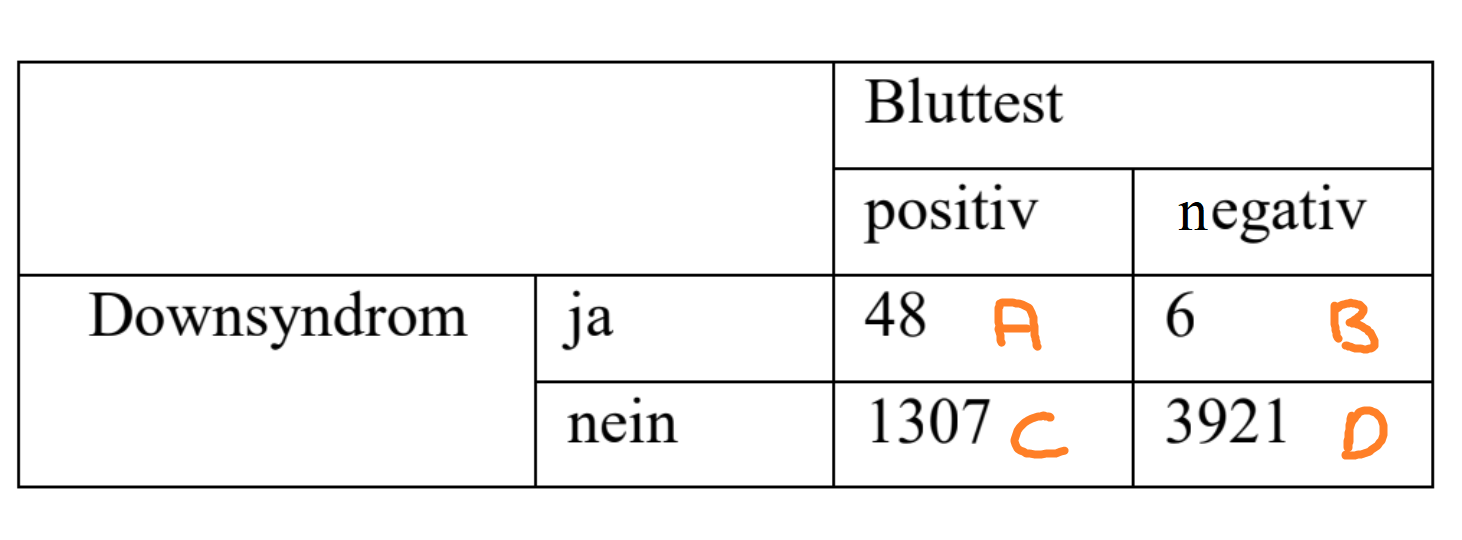
\includegraphics[width=\textwidth]{tabelle4.png}
\vfill
\textbf{Berechnung der Risk-Ratio (Risiko-Verhältnis):}
\begin{align*}
	\text{Risk-Ratio} = \frac{\text{Erkrankungsrisiko mit Risikofaktor}}{\text{Erkrankungsrisiko ohne Risikofaktor}} =  \frac{\frac{A}{A+C}}{\frac{B}{B+D}} = \frac{\frac{48}{48+1307}}{\frac{6}{6+3921}} \approx 23,2
\end{align*}
\end{frame}

\begin{frame}
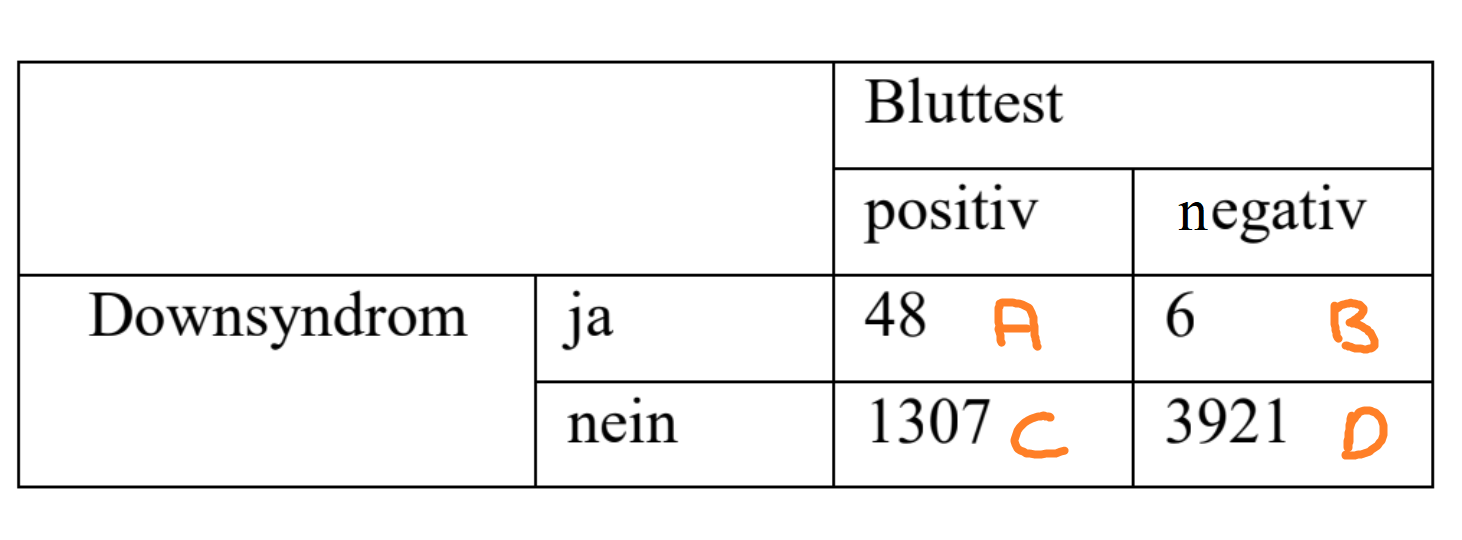
\includegraphics[width=\textwidth]{tabelle4.png}
\vfill
Wichtiger \textbf{Unterschied} zwischen \textbf{Odds-Ratio} und \textbf{Risk-Ratio}: Die Risk-Ratio darf nicht berechnet werden, wenn die Randhäufigkeiten für die Erkrankung festgelegt sind (case-control study). In einem solchen Fall wird die Odds-Ratio berechnet. 
\end{frame}

\begin{frame}
\textbf{Berechnung der Risk-Ratio (Risiko-Verhältnis):}
\begin{align*}
\text{Risk-Ratio} = \frac{\frac{A}{A+C}}{\frac{B}{B+D}} = \frac{\frac{48}{48+1307}}{\frac{6}{6+3921}} \approx 23,2
\end{align*}
\textbf{Interpretation:}
\begin{itemize}
	\item Die Risk-Ratio ist ein Maß dafür, um wie viel größer das \textbf{Risiko} in der Gruppe mit Risikofaktor ist, zu erkranken, verglichen mit dem \textbf{Risiko} in der Gruppe ohne Risikofaktor.
	\item Die Risk-Ratio liegt im Bereich $0$ bis $\infty$.
	\item Eine Risk-Ratio von $1$ bedeutet ein gleiches Risiko.
	\item Eine Risk-Ratio $<1$ bzw. $>1$ bedeutet, dass das Risiko in der ersten Gruppe kleiner bzw. größer ist.
	\item Je weiter die Risk-Ratio von 1 entfernt ist, desto stärker ist der Zusammenhang.
\end{itemize}
\pause
\vfill
\textbf{In unserem Beispiel:} Das Risiko für das Downsyndrom ist bei einem positiven Bluttest 23,2mal so hoch wie bei einem negativen Bluttest.
\end{frame}

\end{document}